%% UzK - A BEAMER THEME FOR THE UNIVERSITY OF COLOGNE
%% http://solstice.github.com/uzk-theme/

\documentclass{beamer}
\usepackage[ngerman]{babel}
%\usepackage[latin1]{inputenc}
\usepackage[T1]{fontenc}
\usepackage{xltxtra} 
\usepackage{wasysym}
\defaultfontfeatures{Mapping=tex-text}


%% Falls Anzeige der \sections, \subsections etc. gewuenscht, kann zB.
%% das infolines theme geladen werden. Wichtig ist jedoch, dass andere
%% Themes _vor_ dem UzK-Theme geladen werden.
%\useoutertheme{infolines}

%% Falls keine der Optionen zur Bestimmung der Fusszeile uebergeben werden    %%
%% werden alle Fakultaetsfarben verwendet. ---------------------------------- %%
\usetheme[%
%wiso,        %% Wiso-Fakultaet
%jura,        %% Rechtswissenschaftliche Fakultaet
medizin,     %% Medizinische Fakultaet
%philo,       %% Philosophische Fakultaet
%matnat,      %% Mathematisch-Naturwissenschaftliche Fakultaet
%human,       %% Humanwissenschaftliche Fakultaet
%verw,        %% Universitaetsverwaltung
%nav,         %% Schaltet die Navigationssymbole ein
%latexfonts,  %% Verwendet die latex-beamer-Standardschrift
%colorful,    %% Farbige Balken im infolines-Theme
%squares,     %% Aufzaehlungspunkte rechteckig
]{UzK}

\title{(Geo)Kettle -- Ein unvollständiger, subjektiver Erlebnisbericht}

\author[Stefan Ziegler]%
{Stefan Ziegler}%
  

\institute[Amt für Geoinformation]{%
Amt für Geoinformation \\
Rötistrasse 4\\
4500 Solothurn}

\date[xx.01.13]{xx. Januar 2014}
\begin{document}

\begin{frame}
  \titlepage
\end{frame}

\begin{frame}
  \frametitle{Inhalt}
  \begin{itemize}
  \item Was ist Kettle? Was ist PDI? Was ist Geokettle?
  \item 
  \item Geo ohne GeoKettle?
  \item Demo
  \item Inspiration
  \end{itemize}
\end{frame}

\begin{frame}
  \frametitle{Kettle/PDI}
  \begin{itemize}
  \item ETL-Tool (Extract, Transform, Load)
  \item Kettle $=$ PDI (Pentaho Data Integration) 
  \item Dual-licensing
  \end{itemize}
\end{frame}

\begin{frame}
  \frametitle{Funktionsweise}
  \begin{itemize}
  \item Hübsche Oberfläche
  \item Relativ intutiv\ldots{}
  \item Prozesse gespeichert in einer XML-Datei (in DB-Repo oder filebasiert)
  \item Kettle \textsl{interpretiert} XML-Datei
  \item Prozess steuerbar mit Parameter und Variablen.
  \item Prozesse werden gestartet:
	  \begin{itemize}
	  \item aus der Oberfläche \textsl{Spoon}
	  \item von der Kommandozeile \textsl{Pan} resp. \textsl{Kitchen}
	  \item via Webserver \textsl{Carte} (auf entferntem Rechner)
	  \item oder ganz abgefahren in Cluster.
	  \end{itemize}
  \end{itemize}
\end{frame}



\begin{frame}
  \frametitle{Weitere ETL-Tools}
  \begin{itemize}
  \item Talend Open Studio (TOS):
	  \begin{itemize}
	  \item komplizierter?
	  \item Codegenerator: Erzeugt Java-Code.
	  \end{itemize}
  \item FME:
	  \begin{itemize}
	  \item Kenne ich nicht.
	  \item Arbeitsplatzwechsel resp. Arbeitsmittelwechsel notwendig \frownie{} 
	  \item Interlis \smiley{} 
	  \end{itemize}

  \end{itemize}
\end{frame}


\begin{frame}
  \frametitle{GeoKettle}
  \begin{itemize}
  \item Kettle um Geoprozesse erweitert.
  \item «Geo» \textsl{nicht} als Plugin integriert.
  \item GeoKettle basiert auf Kettle 3 (aktuell Kettle 5).
  \item aber\ldots{}
  \end{itemize}
\end{frame}

\begin{frame}
  \frametitle{Geo ohne GeoKettle}
  \begin{itemize}
  \item Sämtliche Geoprozesse werden in der Datenbank gemacht.
  \item Funktioniert tadellos aber einschränkend, da z.\,B. kein Import/Export von Shape-Dateien etc. möglich ist.
  \item Beispiele:
  \begin{itemize}
   \item Bodenbedeckungsarten pro Liegenschaft (im öffentlichen Eigentum)
   \item AV-Fileverifikation
  \end{itemize}
 \end{itemize}
\end{frame}


\begin{frame}
  \frametitle{Persönliches Fazit}
  \begin{itemize}
  \item Keine eierlegende Wollmilchsau.
  \item Oftmals reicht wahrscheinlich auch ein Skript.
  \item GeoKettle, quo vadis?
 \end{itemize}
  \begin{itemize}
  \item Fexibel: läuft auch als Cronjob.
  \item Übersichtliches GUI: einzelne Prozessschritte sind klar sichtbar.
  \item Tiefe Hemmschwelle: man programmiert nicht.
  \item Grosse Auswahl an Werkzeugen: E-Mail-Versand, Logging, Access/Excel In-/Output, SAP-Input (?) etc.
 \end{itemize}
\end{frame}


\begin{frame}
  \frametitle{QGIS-GUI}
  \begin{figure}
    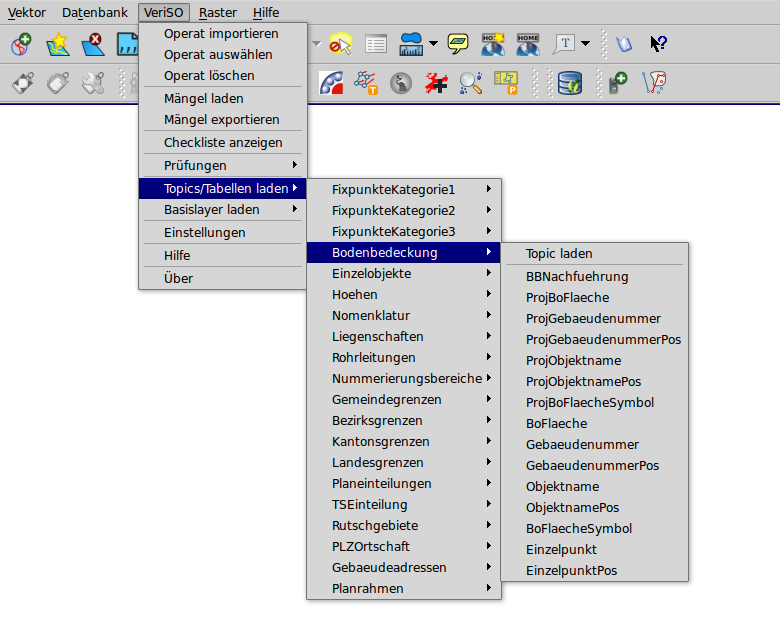
\includegraphics[scale=0.35]{bilder/veriso_topic_loader_3.png}
  \end{figure}
\end{frame}

\begin{frame}
  \frametitle{QGIS-GUI}
  \begin{figure}
    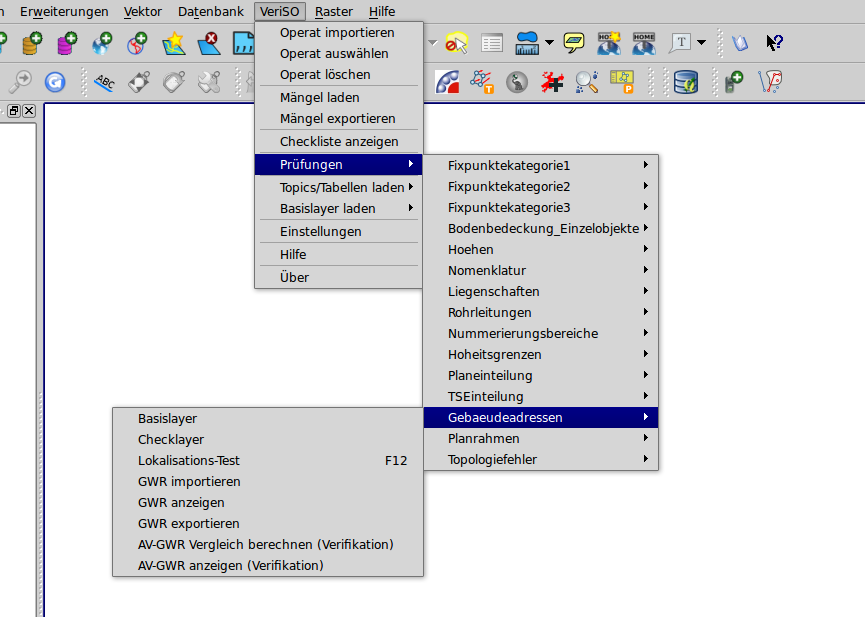
\includegraphics[scale=0.35]{bilder/veriso_checks_3.png}
  \end{figure}
\end{frame}

\begin{frame}[fragile]
  \frametitle{QGIS-GUI: ILI $\rightarrow$ XML}
  \begin{tiny}
  \begin{verbatim}
<?xml version="1.0" encoding="ISO-8859-1"?>
<topics>
  <topic id="FixpunkteKategorie1" title="FixpunkteKategorie1" group="FixpunkteKategorie1">
    <table>
      <group>FixpunkteKategorie1</group>
      <title>LFP1Nachfuehrung</title>
      <schema>av_dm01avso24</schema>
      <table>fixpunktekategorie1_lfp1nachfuehrung</table>
      <geom>perimeter</geom>
      <style></style>
    </table>
    <table>
      <group>FixpunkteKategorie1</group>
      <title>LFP1</title>
      <schema>av_dm01avso24</schema>
      <table>fixpunktekategorie1_lfp1</table>
      <geom>geometrie</geom>
      <style></style>
    </table>
    ....
  <topic id="Bodenbedeckung" title="Bodenbedeckung" group="Bodenbedeckung">   
    <table>
      <group>Bodenbedeckung</group>
      <title>BoFlaeche</title>
      <schema>dm01avso24</schema>
      <table>bodenbedeckung_boflaeche</table>
      <geom>geometrie</geom>
      <style></style>
    </table>
    ....
 </topic>
</topics>    
  \end{verbatim}
  \end{tiny}
\end{frame}


\begin{frame}[fragile]
  \frametitle{QGIS-GUI: XML für Checks}
  \begin{tiny}
  \begin{verbatim}
<?xml version="1.0" encoding="ISO-8859-1"?>
<checks>
  <check id="fixpunktekategorie1" title="Übersicht" group="Fixpunktekategorie1" 
         topic="Fixpunktekategorie1" type="complex">
    <file>complexchecks.fp1</file>
  </check>
  ...  
  <check id="gebaeudeadressen_basis" title="Basislayer" group="Gebaeudeadressen - Basislayer" 
         topic="Gebaeudeadressen" type="complex">
    <file>complexchecks.gebaeudeadressen_basislayer</file>
  </check>   
  <check id="gebaeudeadressen_check" title="Checklayer" group="Gebaeudeadressen - Checklayer" 
         topic="Gebaeudeadressen" type="complex">
    <file>complexchecks.gebaeudeadressen_checklayer</file>
  </check>    
  <check id="gebaeudeadressen_lokalisations" title="Lokalisations-Test" 
         group="Gebaeudeadressen - Lokalisations-Test" topic="Gebaeudeadressen" type="complex">
    <file>complexchecks.gebaeudeadressen_lokalisation</file>
    <shortcut>F12</shortcut>
  </check>           
  ...
</checks>   
  \end{verbatim}
  \end{tiny}
\end{frame}

\begin{frame}[fragile]
  \frametitle{Checks}
  \begin{itemize}
  \item «Alles ist möglich!»
  \item «einfach»:
  \begin{itemize}
   \item Vordefinierte PostGIS-Views oder Tabellen (falls View zu langsam).
   \item Tabellen werden während des Importes abgefüllt.
   \item Queries sind in spezieller Tabelle gespeichert. 
  \end{itemize}
  \item «komplex»:
  \begin{itemize}
   \item beliebig kompliziert
   \item Alles was die Python- und PyQGIS-API hergibt, z.\,B.:
   \begin{itemize}
    \item Excel-Export
    \item PDF erzeugen
    \item Daten mit WFS requesten und vergleich.
    \item \ldots
   \end{itemize}

  \end{itemize}
  
  \item Alles in \textit{mindestens} einer Python-Datei verpackt.
 \end{itemize}
\end{frame}

\begin{frame}
  \frametitle{Checks}
  \begin{figure}
    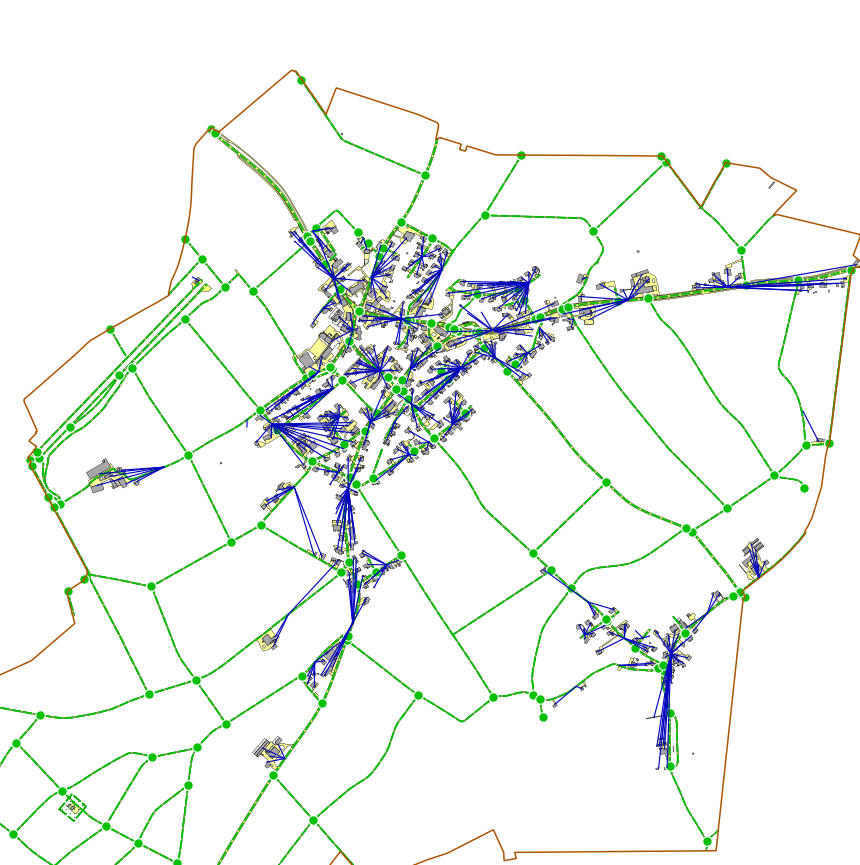
\includegraphics[scale=0.3]{bilder/veriso_spinnennetz_1.png}
  \end{figure}
\end{frame}

\begin{frame}
  \frametitle{Checks}
  \begin{figure}
    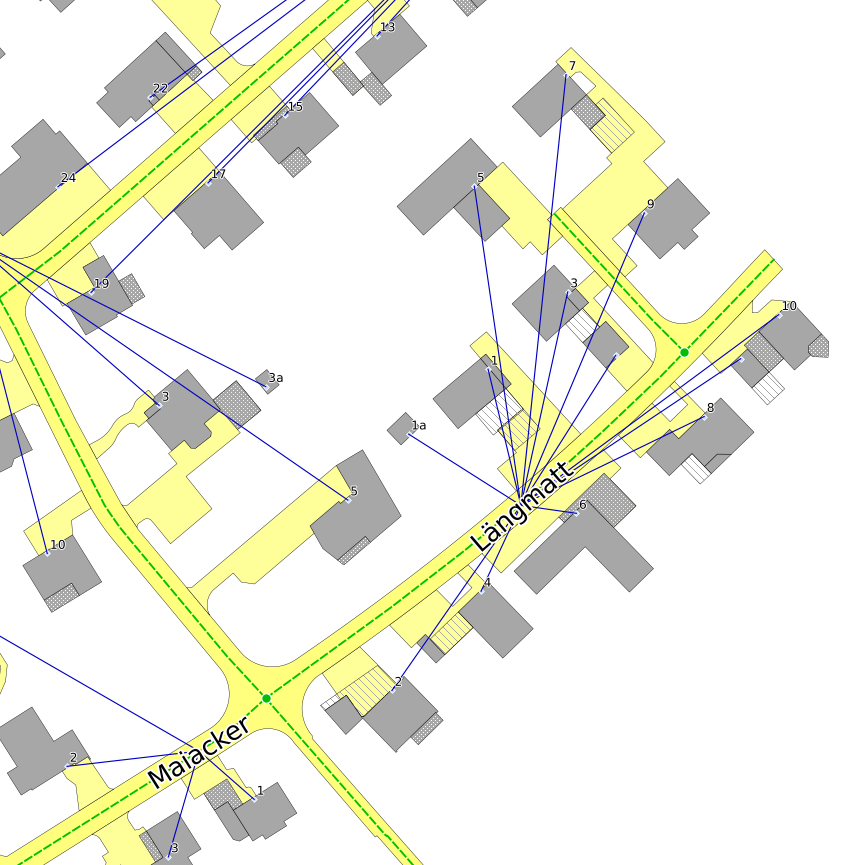
\includegraphics[scale=0.3]{bilder/veriso_spinnennetz_2.png}
  \end{figure}
\end{frame}

\begin{frame}
  \frametitle{Checks}
  \begin{figure}
    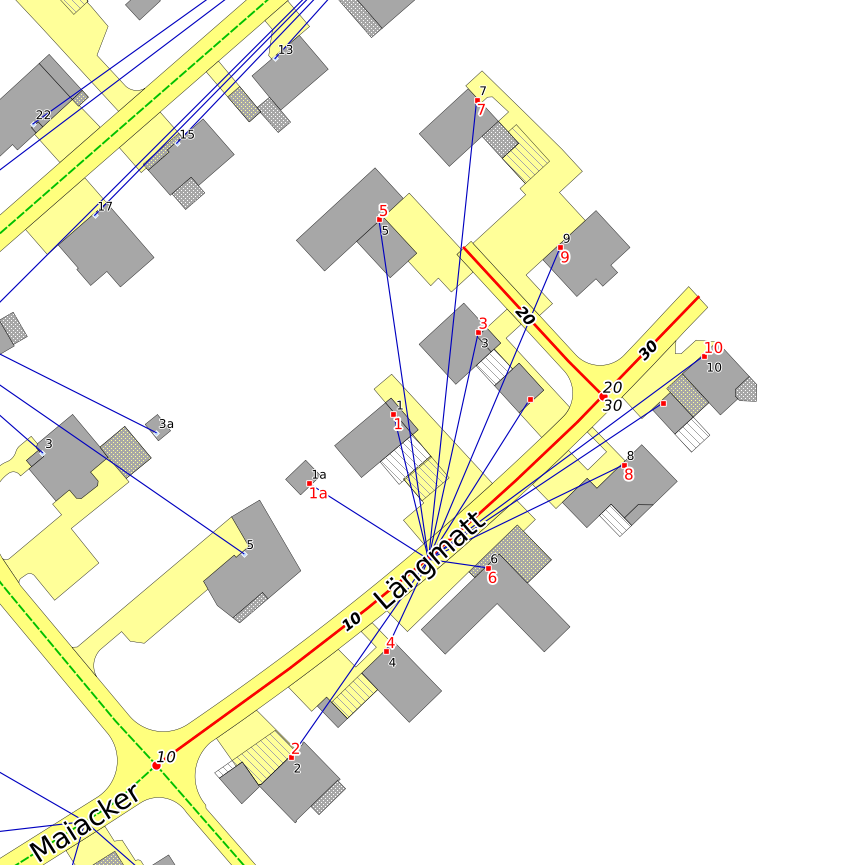
\includegraphics[scale=0.3]{bilder/veriso_f12.png}
  \end{figure}
\end{frame}

\begin{frame}
  \frametitle{Checks}
  \begin{figure}
    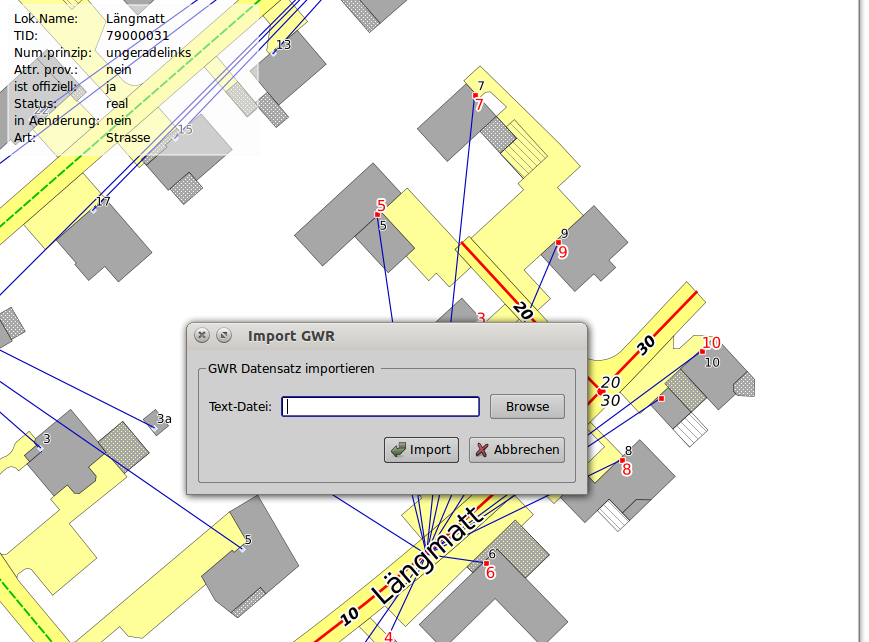
\includegraphics[scale=0.3]{bilder/veriso_gwr_import.png}
  \end{figure}
\end{frame}

\begin{frame}[fragile]
  \frametitle{Checks: Umsetzung GUI}
  \begin{tiny}
  \begin{verbatim}
<?xml version="1.0" encoding="ISO-8859-1"?>
<checks>
  <check id="fixpunktekategorie1" title="Übersicht" group="Fixpunktekategorie1" 
         topic="Fixpunktekategorie1" type="complex">
    <file>complexchecks.fp1</file>
  </check>
  ...  
  <check id="gebaeudeadressen_basis" title="Basislayer" group="Gebaeudeadressen - Basislayer" 
         topic="Gebaeudeadressen" type="complex">
    <file>complexchecks.gebaeudeadressen_basislayer</file>
  </check>   
  <check id="gebaeudeadressen_check" title="Checklayer" group="Gebaeudeadressen - Checklayer" 
         topic="Gebaeudeadressen" type="complex">
    <file>complexchecks.gebaeudeadressen_checklayer</file>
  </check>    
  <check id="gebaeudeadressen_lokalisations" title="Lokalisations-Test" 
         group="Gebaeudeadressen - Lokalisations-Test" topic="Gebaeudeadressen" type="complex">
    <file>complexchecks.gebaeudeadressen_lokalisation</file>
    <shortcut>F12</shortcut>
  </check>           
  ...
</checks>   
  \end{verbatim}
  \end{tiny}
\end{frame}

\begin{frame}
  \frametitle{Checks: Umsetzung GUI}
  \begin{figure}
    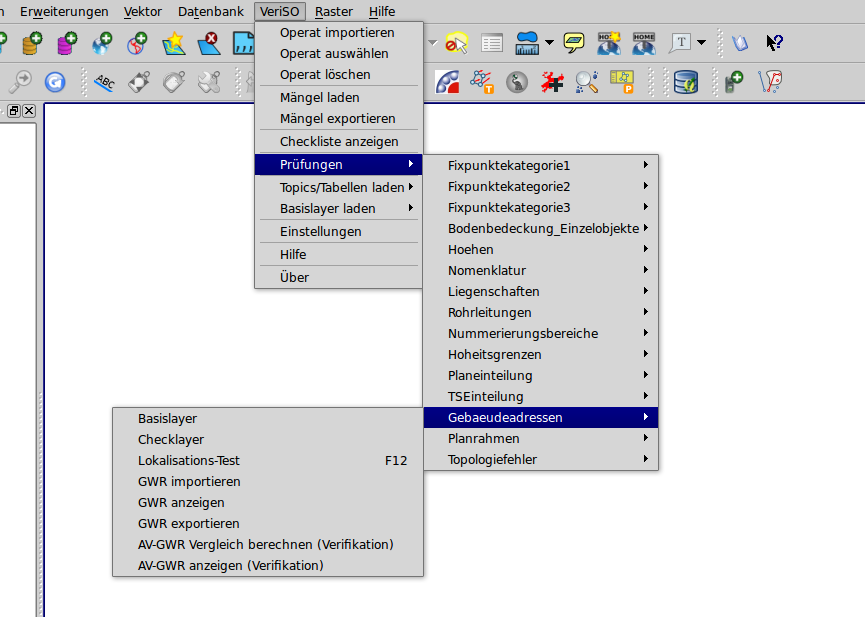
\includegraphics[scale=0.35]{bilder/veriso_checks_3.png}
  \end{figure}
\end{frame}




\begin{frame}[fragile]
  \frametitle{Checkliste}
  \begin{itemize}
  \item Möglichst einfach.
  \item Keine zusätzliche Software.
  \item HTML-Formulare
  \item Persistentes Speichern von Daten mittels \textit{Web Storage}.
  \item Achtung: Daten «nur» im Browser gespeichert!
  \item Für jedes Operat wird HTML-Datei von Template kopiert.
  \end{itemize}
\end{frame}





\end{document}
